\chapter{I2C Real Time Clock}

\section{Configuration}
The Beaglebone series of development boards does not include a ``real time clock'' with a battery back-up.  The included real time clock only functions while power is applied to the board.

When a Linux based device has connectivity to the internet, it can access the current time via ``Network Time Protocol'' (NTP).  These are servers which are maintained with very precise timing.

The Debian distribution used with the BBGW includes NTP already up and running.  The Beaglebone's own real time clock is synchronized using NTP at boot.  However, if boot occurs with no access to internet, the real time clock will have a large error.

A hardware ``real time clock'' (RTC) can be added to provide accurate timing to the board even if the internet connection is down.  A lithium battery powers the RTC even when power is removed from the BBGW.

If the home system has consistent power and the wireless is never turned off, adding a real time clock will not provide a benefit.  In fact, the RTC included with the BBGW may be adequate for most applications even with intermittent internet connection.  This project's timing controller does not save to non-volatile memory, and timing events will be lost in case of a power failure.  Addition of a battery powered external real time clock will benefit systems which rarely or never have access to the internet.

Please note that this subject of time, date, and clocks can get quite complex!  Linux has several mechanisms and services for tracking date and time and keeping everything synchronized, and this can get rather confusing.  Reading the manual pages for ``hwclock'' and ``timedatectl'' is highly encouraged.  Read the discussion in this link to get an idea of the complexities of Linux and RTCs:

\url{https://bugs.debian.org/cgi-bin/bugreport.cgi?bug=785445}

The following real time clock module is suggested:

\url{https://www.seeedstudio.com/Grove-High-Precision-RTC-p-2741.html}

\begin{figure}[H]
	\centering
	
\includegraphics[width=0.6\textwidth]{photos/grove-rtc}
	\centering\bfseries
	\caption{Seeed Studio's Grove High Precision RTC}
\end{figure}

The clock has a ``Grove'' connector and cable and easily plugs into the BBGW.  A kernel driver exists for this device and is included with the Beagleboard Debian distributions.

You will need to purchase a CR1225 3.3 volt coin cell battery.  This is a less-common cell which may have to be mail ordered.

Install the battery in the RTC, and plug it into the I2C Grove connector on the BBGW.  This is the Grove connector closest to P9.  The other Grove connector is for UART.

Power up the BBGW and log in.  Try this command at the command line:

\begin{verbatim}
i2cdetect -y -r 2
\end{verbatim}

You should see this:

\begin{verbatim}
     0  1  2  3  4  5  6  7  8  9  a  b  c  d  e  f
     00:          -- -- -- -- -- -- -- -- -- -- -- -- -- 
     10: -- -- -- -- -- -- -- -- -- -- -- -- -- -- -- -- 
     20: -- -- -- -- -- -- -- -- -- -- -- -- -- -- -- -- 
     30: -- -- -- -- -- -- -- -- -- -- -- -- -- -- -- -- 
     40: -- -- -- -- -- -- -- -- -- -- -- -- -- -- -- -- 
     50: -- 51 -- -- UU UU UU UU -- -- -- -- -- -- -- -- 
     60: -- -- -- -- -- -- -- -- -- -- -- -- -- -- -- -- 
     70: -- -- -- -- -- -- -- --
\end{verbatim}

The above output from i2cdetect indicates the RTC is successfully installed and communicating via I2C bus.

Now ``install'' the I2C device with this command:

\begin{verbatim}
sudo sh -c 'echo pcf85063 0x51 > /sys/class/i2c-adapter/i2c-2/new_device'
\end{verbatim}

Now see if the real time clock installed successfully:

\begin{verbatim}
cat /sys/class/rtc/rtc1/name
\end{verbatim}

This should return:

\begin{verbatim}
rtc-pcf85063
\end{verbatim}

There should also be a new device appear at /dev/rtc1.  There are also /dev/rtc which is a link to /dev/rtc0.  rtc0 is the BBGW's own internal RTC.

Now read back the time from the new RTC:

\begin{verbatim}
sudo hwclock -r -f /dev/rtc1
\end{verbatim}

You will probably get something like this:

\begin{verbatim}
Sat 01 Jan 2000 12:24:47 AM EST  -0.582551 seconds
\end{verbatim}

Now the RTC must be ``set''.  The following assumes that the BBGW is connected to the internet, and it is using the ``Network Time Protocol'' service which was implemented by default in the image used for this project.
To check this, use this command:

\begin{verbatim}
timedatectl
\end{verbatim}

This will return something like this:

\begin{verbatim}
      Local time: Sat 2017-07-15 19:24:20 EDT
      Universal time: Sat 2017-07-15 23:24:20 UTC
      RTC time: Sat 2017-07-15 23:24:21
      Time zone: America/New_York (EDT, -0400)
      Network time on: yes
      NTP synchronized: yes
      RTC in local TZ: no
\end{verbatim}

This indicates that the automatic synchronization to NTP is enabled.
Note that the ``RTC time'' is the BBGW's own internal RTC.  ``Local time'' and ``Universal time'' are both derived from the ``system time''.  ``System time'' is what the microcontroller actually uses, so it is system time which is ultimately desired to be set accurately.  System time is typically set at boot via some accurate source like that from NTP or an RTC.

Now write the system time to the external RTC.  This should be accurate if the BBGW is connected to the internet.

\begin{verbatim}
sudo hwclock -w --rtc /dev/rtc1
\end{verbatim}

Note the override --rtc option in the above command.  Please see the hwclock man page for an explanation of this option.

Now read the real time clock to verify it is accurately set:

\begin{verbatim}
hwclock -r --rtc /dev/rtc1
\end{verbatim}

The time returned above can be compared to the ``date'' command.

The above process will not be preserved upon next boot-up.  It is necessary to create a ``service'' and start it each time the board is booted.  Fortunately this is simple to accomplish.

A bash script which duplicates the set-up described above is included in the software directory:

\begin{verbatim}
#!/bin/bash

echo 'pcf85063 0x51' > /sys/class/i2c-adapter/i2c-2/new_device
hwclock -s --rtc /dev/rtc1 --debug
hwclock --adjust --rtc /dev/rtc1
\end{verbatim}

The above script is in the github repository with path software/systemd/real-time-clock-init.sh.

Next, a systemd service must be established to run the script and synchronize the system clock at boot:

\begin{verbatim}
[Unit]
Description=PCF85063 RTC Service

[Service]
Type=simple
WorkingDirectory=/home/debian/irrigate-control/software/systemd
ExecStart=/bin/bash real-time-clock-init.sh
SyslogIdentifier=real_time_clock

[Install]
WantedBy=graphical.target
\end{verbatim}

The file is located in the github repository at software/systemd/real-time-clock.service.
Copy this as follows:

\begin{verbatim}
sudo cp real-time-clock.service /etc/systemd/system
\end{verbatim}

Now the service must be enabled:

\begin{verbatim}
sudo systemctl enable real-time-clock
\end{verbatim}

One last bit of configuration is required.  The RTC kernel module must be added to the /etc/modules file.  Simply add this line to the file:

\begin{verbatim}
rtc-pcf85063
\end{verbatim}

Reboot after all of the above configuration is complete.  If all is well, the hwclock -r command as shown above should show good absolute time accuracy.  The RTC should show up as device /dev/rtc1 and also by using the command lsmod, the driver rtc\_pcf85063 should be listed.

To see the status of the real-time-clock service, use this command:

\begin{verbatim}
systemctl status real-time-clock
\end{verbatim}

The above command will print current status of the service as well as error messages if the service has malfunctioned.

\section{RTC Hardware Installation}

Thanks to the Grove connector system the installation of the RTC is easy.

A Grove I2C hub was used, as this allows other devices to be added to the I2C bus in the future:

\url{https://www.seeedstudio.com/Grove-I2C-Hub-p-851.html}

Both the hub and the RTC were mounted using electronic grade silicone adhesive.  Do not use ordinary RTV!  The usual hardware store RTV contains acid which will damage electronics.

\begin{figure}[H]
	\centering
	
\includegraphics[width=0.7\textwidth]{photos/silicone}
	\centering\bfseries
	\caption{Electronics Grade Silicone Adhesive}
\end{figure}

The mounting surface should be clean.  Coat the bottom surface of the boards and lightly press them onto the desired location.  Wait about two hours for the silicone to firm up, and then install the cable assemblies.  Be sure to plug into the Grove I2C connector on the BBGW, not the UART.

\begin{figure}[H]
	\centering
	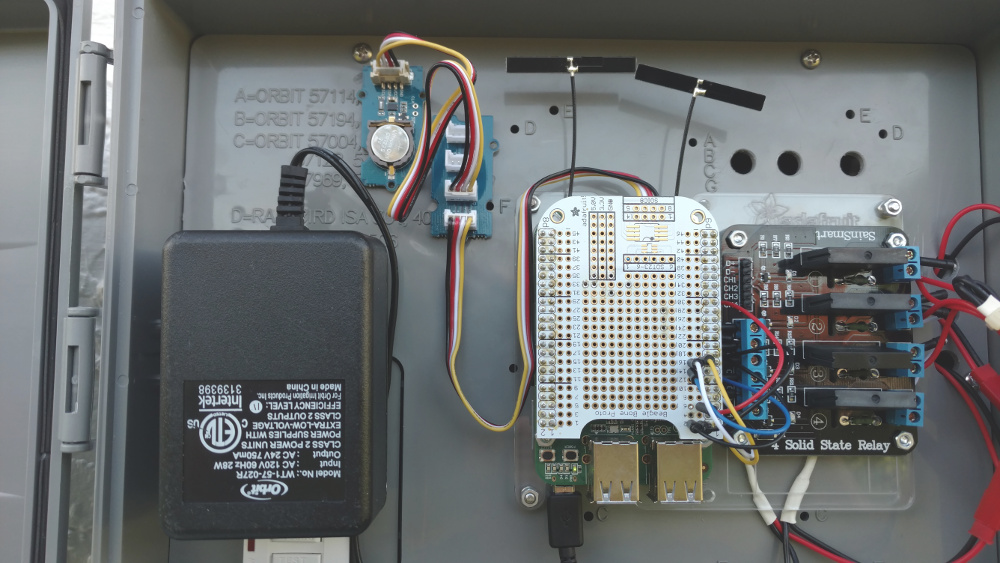
\includegraphics[width=0.7\textwidth]{photos/rtc-mounted}
	\centering\bfseries
	\caption{Grove Hub and Precision RTC Mounted in the Weatherproof Enclosure}
\end{figure}


